%
\documentclass[12pt]{article}

\usepackage{fullpage}
\usepackage{setspace}
\usepackage{endnotes}
\usepackage{amsmath}
\usepackage{amsfonts}
\usepackage{amssymb}
\usepackage{calrsfs}
\usepackage{rotating}
\usepackage{dcolumn}
\usepackage{longtable}
\usepackage{microtype}
\usepackage{graphicx}
\usepackage{url}
\usepackage{natbib}
\bibpunct{(}{)}{;}{a}{}{,}
\usepackage{framed}
\usepackage{lipsum}
\usepackage[font=small,labelfont=sc]{caption}
 \usepackage{float}
\restylefloat{table}
\usepackage[usenames,dvipsnames]{color}

% refs and pdf meta
\usepackage{hyperref}
\hypersetup{
 pdftitle={Reasonable Measures of Uncertainty Under Separation}, % title
 pdfauthor={Carlisle Rainey}, % author
 pdfkeywords={logistic regression}{separation}{Firth}{Cauchy}{MCMC}
 pdfnewwindow=true, % links in new window
 colorlinks=true, % false: boxed links; true: colored links
 linkcolor=BrickRed, % color of internal links
 citecolor=BrickRed, % color of links to bibliography
 filecolor=BrickRed, % color of file links
 urlcolor=BrickRed % color of external links
}

% Set up theorems, etc.
\usepackage{amsthm}
\newtheorem{lemma}{Lemma}
\newtheorem{proposition}{Proposition}
\newtheorem{theorem}{Theorem}
\newtheorem{claim}{Claim}
\newtheorem{assumption}{Assumption}

% Allow restating theorems (for the Appendix)
\usepackage{thmtools}
\usepackage{thm-restate}
\usepackage{cleveref}


% Set up fonts the way I like
\usepackage{tgpagella}
\usepackage[T1]{fontenc}
%\usepackage[T1]{fontenc}
\usepackage[bitstream-charter]{mathdesign}


%Redefine the first level
\renewcommand{\theenumi}{\arabic{enumi}.}
\renewcommand{\labelenumi}{\theenumi}
%Redefine the second level
\renewcommand{\theenumii}{\alph{enumii}.}
\renewcommand{\labelenumii}{\theenumii}
%Redefine the third level
\renewcommand{\theenumiii}{\roman{enumiii}.}
\renewcommand{\labelenumiii}{\theenumiii}
%Redefine the fourth level
\renewcommand{\theenumiv}{\Alph{enumiv}.}
\renewcommand{\labelenumiv}{\theenumiv}


\parskip=0pt
\parindent=20pt
\usepackage{lscape}
\singlespace

% Create footnote command so that my name
% has an asterisk rather than a one.
\long\def\symbolfootnote[#1]#2{\begingroup%
\def\thefootnote{\fnsymbol{footnote}}\footnote[#1]{#2}\endgroup}

\begin{document}


\begin{center}
{\LARGE Reasonable Measures of Uncertainty Under Separation\symbolfootnote[1]{I thank [many people]. Thanks to Mark Bell and Nicholas Miller for making their data available to me. The analyses presented here were conducted with \texttt{R} 3.1.0 and JAGS 3.3.0. All data and computer code necessary for replication are available at \href{https://github.com/carlislerainey/priors.for-separation}{github.com/carlislerainey/priors-for-separation}.}}

\vspace{10mm}

Carlisle Rainey\symbolfootnote[2]{Carlisle Rainey is Assistant Professor of Political Science, University at Buffalo, SUNY, 520 Park Hall, Buffalo, NY 14260 (\href{mailto:rcrainey@buffalo.edu}{rcrainey@buffalo.edu}).}

\end{center}

% remove page number from first page
\thispagestyle{empty}

% abstract
\vspace{10mm}
{\centerline{\textsc{Abstract}}}
\begin{quote}\noindent When facing data sets with small numbers of observations or ``rare events,'' political scientists often encounter important explanatory variables that perfectly predict binary events or non-events. In this situation, maximum likelihood provides implausible estimates and the researcher must incorporate some form of prior information in the estimation. The most sophisticated research uses Jeffreys' invariant prior to stabilize the estimates. While Jeffreys' prior has the advantage of being automatic, I show that, in many cases, it offers too much prior information, providing confidence intervals that are much too narrow. I show that the choice of a more reasonable prior can lead to different substantive conclusions about the likely magnitude of an effect and I offer practice advice for choosing a prior distribution that represents actual prior information.\end{quote}


\newpage
\doublespace

\section*{The Logistic Regression Model}

Political scientists commonly use logistic regression to model the probability of an event of interest. In the typical situation, the researcher uses an $n \times (k + 1)$ design matrix $X$ consisting of an intercept and $k$ covariates to model a vector $n$ of binary outcomes $y$, where $y_i \in \{0, 1\}$ using the model $\text{Pr}(y_i) = \text{Pr}(y_i = 1 | X_i) = \dfrac{1}{1 + e^{-X_i\beta}}$, where $\beta$ is a parameter vector of length $k + 1$. 

Using this model, it is straightforward to calculate the likelihood function 

\begin{equation}\nonumber
\text{Pr}(y | \beta) = L(\beta | y) = \displaystyle \prod_{i = 1}^n \left[\left( \dfrac{1}{1 + e^{-X_i\beta}}\right)^{y_i} + \left( \dfrac{1}{1 + e^{-X_i\beta}}\right)^{1 - y_i}\right]\text{.}
\end{equation}

\noindent As usual, one can take the natural logarithm of both sides to calculate the log-likelihood function 

\begin{equation}\nonumber
\log L(\beta | y) = \displaystyle \sum_{i = 1}^n \left[y_i \log \left( \dfrac{1}{1 + e^{-X_i\beta}}\right) + (1 - y_i) \log \left( \dfrac{1}{1 + e^{-X_i\beta}}\right)\right]
\end{equation}

\noindent and take the derivatives of the log-likelihood function to obtain the score function

\begin{equation}\nonumber
\dfrac{\partial \log L(\beta | y)}{\partial \beta} = \displaystyle \sum_{i = 1}^n\left(y_i - \dfrac{1}{1 + e^{-X_i\beta}}\right)X_i\text{.}
\end{equation}

Researchers routinely obtain maximum likelihood estimates $\hat{\beta}^{mld}$ of the model parameters $\beta$ by setting the score function equal to zero and solving for $\beta$ (i.e., maximizing the likelihood of the observed data) and estimate the standard errors are by calculating the square root of the diagonal of the inverse of Fisher's information matrix evaluated at $\hat{\beta}^{mle}$ (i.e., calculate the curvature around the maximum of the likelihood function to obtain an estimate of the uncertainty of the estimate). While this approach works quite well in most applications, it fails in a situation known as separation \citep{Zorn2005}.

\section*{Separation}

Separation occurs in models of binary outcome data when one explanatory variable (or perhaps a combination of explanatory variables, see \cite{LesaffreAlbert1989}) perfectly predicts zeros, ones, or both. \textit{Complete separation} occurs when the ``problematic'' explanatory variable $s_i$ (for \underline{s}eparating explanatory variable) perfectly predicts both zeros and ones and \textit{quasicomplete separation} occurs when $s_i$ perfectly predicts either zeros or ones, but not both (\citealt{AlbertAnderson1984, Zorn2005}). \textit{Overlap}, the ideal case, occurs when there is no such $s_i$ that perfectly predicts zeros or ones.\footnote{[tk: cite] explain that combinations of explanatory variables can also produce separation, but I focus here on single separating explanatory variables.} In this situation, the usual maximum likelihood estimates exist and provide reasonable estimates of parameters. However, under complete or quasicomplete separation, maximum likelihood estimates do not exist (\citealt{AlbertAnderson1984, Zorn2005}).

Complete separation occurs when a covariate perfectly predicts zeros and ones. For example, suppose an explanatory variable $s_i$ , such that $y_i = 0$ for $s_i > 0.5$ and $y_i = 0$ for $s_i \leq 0.5$. This corresponds to the middle panel of Figure \ref{fig:illustrating_separation}.  To maximize the likelihood of the observed data, the ``S''-shaped logistic regression curve must assign probabilities of zero when $s_i \leq 0.5$ and probabilities of one when $s_i > 0.5$. Since the logistic regression curve lies strictly between zero and one, this likelihood cannot be achieved. However, it can be approached asymptotically as the coefficient for $s_i$ approaches infinity. Thus, the likelihood function under complete separation is monotonic (has no maximum) and a finite maximum likelihood estimate does not exist.

Quasicomplete separation occurs when a covariate perfectly predicts zeros \textit{or} ones. Figure \ref{fig:illustrating_separation} shows an example pattern in the right panel, where $y_i$ always equals zero when $s_i$ equals zero. This situation occurs often in applied political science research with binary inputs. For example, \cite{Gelmanetal2008} find no African-American respondents in their data support Barry Goldwater in 1964, leading to a maximum likelihood estimate of negative infinity for the coefficients for the indicator of African-American respondents. Similarly, \cite{Rauchhaus2009} (see \citealt{BellMiller2014}) finds no instances of states with nuclear weapons engaging in war with each other. In this case, the estimated coefficient for the variable indicating symmetric nuclear dyads (in which both states possess nuclear weapons) equals negative infinity. To maximize the likelihood in this situations, the model must assign probabilities of zero to observations for which $s_i = 1$ (African-American respondents or symmetric nuclear dyads, in these examples). Again, because the logistic regression curve lies strictly above zero, this cannot happen, though it can be approached asymptotically as the coefficient for $s_i$ goes to negative infinity. As with complete separation, the likelihood function under quasicomplete separation is monotonic (has no maximum) and a finite maximum likelihood estimate does not exist.

\begin{figure}[H]
\begin{center}
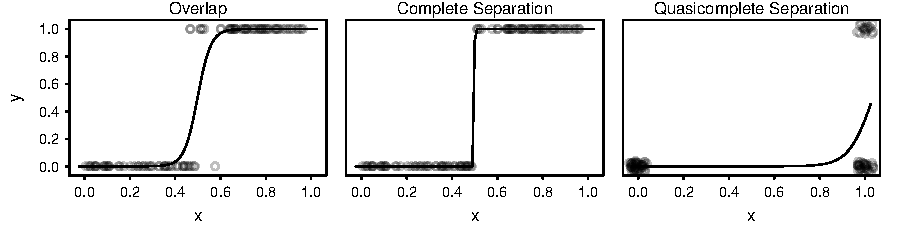
\includegraphics[scale = 1]{figs/illustrate-separation.pdf}
%\vspace{-10mm}
\end{center}
\caption{This figure illustrates overlap, complete separation, and quasicomplete separation as defined by \cite{AlbertAnderson1984}. The maximum likelihood estimates only exist under overlap. Under complete and quasicomplete separation, maximum likelihood fails, returning infinite estimates and standard errors.}\label{fig:illustrating_separation}
\end{figure}

For convenience, I refer to the variable $s_i$ as the ``\underline{s}eparating variable'' and denote its coefficient as $\beta_s$. I also say that the ``direction of the separation'' is positive if and only if $s_i = 1 \implies y_i = 1$ \underline{or} $s_i = 0 \implies y_i = 0$ and that the direction of separation is negative if and only if $s_i = 0 \implies y_i = 1$ \underline{or} $s_i = 1 \implies y_i = 0$. Thus, when the direction of the estimate is positive $\hat{\beta}^{mle} = +\infty$, and when the direction of the estimate is negative $\hat{\beta}^{mle} = -\infty$.

Along coefficient estimates under separation are infinite in theory, the hill-climbing algorithms approximate the infinite estimates with large, finite values that increase with the precision of the algorithm. Table \ref{tab:illustrating_separation} shows the estimates from R's \texttt{glm()} function for each of the hypothetical data sets in Figure \ref{fig:illustrating_separation}. To illustrate the problem, I vary the convergence tolerance between $\epsilon = 10^{-8}$ (the default) and $\epsilon = 10^{-16}$. With the default tolerance, \texttt{glm()} returns very large estimates and standard errors. There is no finite maximum, but the likelihood is flat enough around the large estimates to satisfy the algorithm, given the default tolerance. With the more sensitive tolerance of $\epsilon = 10^{-16}$, the algorithm converges even closer to infinity, but still returns finite estimates. This is a failure of maximum likelihood, because estimates of infinity are usually implausible (i.e., there is always some, though perhaps tiny, probability of a zero or one in any given situation, see \citealt{HeinzeSchemper2002}). 

\begin{table}[H]
\begin{center}
\begin{footnotesize}
\begin{tabular}{l c c | c c | c c }
\hline
 & \multicolumn{2}{c}{Overlap}&\multicolumn{2}{c}{Complete Separation}&\multicolumn{2}{c}{Quasicomplete Separation}\\
               & $\epsilon = 10^{-8}$ & $\epsilon = 10^{-16}$ & $\epsilon = 10^{-8}$ & $\epsilon = 10^{-16}$ & $\epsilon = 10^{-8}$ & $\epsilon = 10^{-16}$ \\
\hline
constant    & $-17.05$ & $-17.05$ & $-739.27$     & $-739.27$     & $-19.57$    & $-26.57$     \\
               & $(5.79)$      & $(5.79)$      & $(139744.58)$ & $(139744.58)$ & $(1520.85)$ & $(50363.70)$ \\
x              & $34.19$  & $34.19$  & $1483.21$     & $1483.21$     & $18.90$     & $25.90$      \\
               & $(11.92)$     & $(11.92)$     & $(280801.40)$ & $(280801.40)$ & $(1520.85)$ & $(50363.70)$ \\
\hline
Log Likelihood & -9.74         & -9.74         & 0.00          & 0.00          & -32.05      & -32.05       \\
Num. obs.      & 100           & 100           & 100           & 100           & 100         & 100          \\
\hline
\multicolumn{7}{l}{Standard errors in parentheses.}
\end{tabular}
\caption{A table providing estimates based on the data shown in Figure \ref{fig:illustrating_separation} using the R function \texttt{glm()} varying the convergence tolerance under overlap, complete separation, and quasicomplete separation. Notice that the estimation algorithm returns estimates and standard errors arbitrarily close to infinity under both types of separation as the tolerances shrinks to zero.}
\label{tab:illustrating_separation}
\end{footnotesize}
\end{center}
\end{table}

Perhaps more starkly, notice  that the strong pattern in the middle panel of Figure \ref{fig:illustrating_separation} does not produce statistically significant result. This is because the likelihood is essentially flat around the ``maximum'' found by the hill-climbing algorithm. As the region around the maximum flattens, the estimates of the standard errors increases. Thus, separation leads to implausible large estimates \textit{and} standard errors. Notice, for example, that while the data in the middle and right panel would almost never occur under the null hypothesis of no relationship, none of the estimates are statistically significant.

\section*{Solutions to Separation}

The maximum likelihood framework (ML) requires the researcher to find the parameter vector that ``maximizes the likelihood of the observed data.'' Of course, infinite coefficients \textit{always} generate separated data, while finite coefficients only generate separation \textit{sometimes}. Thus, under separation, the researcher can only obtain infinite estimates using ML.

Before addressing potential solutions, let me mention two unsatisfactory ``solutions'' found in applied work. In some cases, researchers simply ignore the problem of separation and interpret the large estimates and standard errors as though these are reasonable. However, this approach leads researchers to overstate the magnitude of the effect and the uncertainty of those estimates. A second approach used in practice is to drop the separating variable from the model. \cite{Zorn2005} correctly dismisses this approach:

\begin{quote}
As a practical matter, separation forces the analyst to choose from a number of problematic alternatives for dealing with the problem. The most widely used ``solution'' is simply to omit the offending variable or variables from the analysis. In political science, this is the approach taken in a number of studies in international relations, comparative politics, and American politics. It is also the dominant approach in sociology, economics, and the other social sciences, and it is the recommended method in a few prominent texts in statistics and econometrics. Of course, this alternative is a particularly unattractive one; omitting a covariate that clearly bears a strong relationship to the phenomenon of interest is nothing more than deliberate specification bias.
\end{quote}

As an alternative, \cite{Zorn2005} recommends building prior information $p(\beta)$ into the model using Bayes' rule, so that 

\begin{equation}\nonumber
p(\beta|y) = \dfrac{\overbrace{p(y|\beta)}^{likelihood}\overbrace{p(\beta)}^{prior}}{\int p(y|\beta)p(\beta) d\beta}~\text{.}
\end{equation}

\noindent In this case, the estimate switches to from the maximum likelihood estimate to a summary of the location of the posterior distribution, such as the posterior mode or mean. The current literature on dealing with separation suggests researcher take an automatic approach, adopting Jeffrey's invariant prior distribution.

\subsection*{Jeffrey's Invariant Prior}

\cite{Zorn2005} introduces political scientists to Firth's \citeyear{Firth1993} modified score function (see \citealt{HeinzeSchemper2002} as well). Firth suggests replacing the usual log-likelihood function $\text{log}\,L(\beta | y)$ with a ``penalized'' likelihood function $\text{log}\,L(\beta | y)$, so that $\text{log}\,L^*(\beta | y) = \text{log}\,L(\beta | y)|I(\beta)|^\frac{1}{2}$. It turns out that this penalty is equivalent to Jeffreys' prior for the logistic regression model. The posterior distribution can be obtained by applying Jeffreys' (\citeyear{Jeffreys1946}) rule, which requires setting the prior $p(\beta)$ to be proportional to the square root of the determinant of the information matrix, so that $p(\beta) = |I(\beta)|^\frac{1}{2}$. Then, of course, applying Bayes' rule to obtain the posterior distribution $p(\beta | y) \propto L(\beta | y)|I(\beta)|$, so that Firth's penalty approach is equivalent to a Bayesian approach with Jeffreys' prior.

The usual method of obtaining standard errors is to assume a multivariate normal sampling distribution for the parameter vector $\beta$ and obtain the $(i, j)$ entry of the covariance matrix $\Sigma_\beta$ by calculating the curvature around the maximum likelihood using $\dfrac{\partial^2 \text{log}\,L(\beta | Y)}{\partial \beta_i \partial \beta_j}$ or posterior mode $\dfrac{\partial^2 \text{log}\,\,p(\beta | Y)}{\partial \beta_i \partial \beta_j}$. 

But \citep{HeinzeSchemper2002} and \cite{Zorn2005} point out that this asymptotic approximation of the sampling distribution as normally (symmetrically) distributed might not be appropriate under separation. As an alternative, the suggest using likelihood profiling to obtain the desired confidence interval. They suggest that analysts obtain a $(1 - \alpha)100\%$ confidence interval for the model parameter $\beta_i$ by calculating the (continuous) set of values for which the likelihood-ratio falls below the $(1 - \alpha)100$ percentile of the $\chi^2_1$ distribution \citep{HeinzeSchemper2002}.

However, \cite{Firth1993} did not propose his prior to solve the separation problem. Instead, his purpose was to reduce the well-known small sample bias in logistic regression models. And while it is true that Firth's correction does provide finite estimates under separation, it remains an open question as to whether this automatic prior, designed for other purposes, provides a reasonable estimate of the uncertain of the estimates.

\subsection*{The Cauchy Prior}

Indeed, \cite{Gelmanetal2008} note that Firth's application of Jeffreys' prior is not easily interpretable as an actual application of prior information because the prior $p(\beta) = |I(\beta)|^\frac{1}{2}$. Instead, they suggest an informative prior that, like Jeffreys' prior, bounds the estimates away from positive and negative infinity but has a scale parameter $\sigma$ that allows researchers to choose the amount of prior information provided to the model. They suggest using the Cauchy distribution as priors for the model coefficients.\footnote{Though \cite{Gelmanetal2008} allow for various user-defined prior distributions, they suggest a Cauchy prior centered at zero with scale of 2.5 as a default for appropriately rescaled variables. They suggest rescaling binary inputs to have mean zero and rescaling continuous inputs to have a mean of zero and a standard deviation of one half before estimating the model.}

The Cauchy distribution resembles a normal distribution, but has much heavier tails (it is equivalent to a $t$ distribution with one degree of freedom), which captures the prior belief that the effect is probably smaller, but has some chance of being quite large.

\begin{figure}[H]
\begin{center}
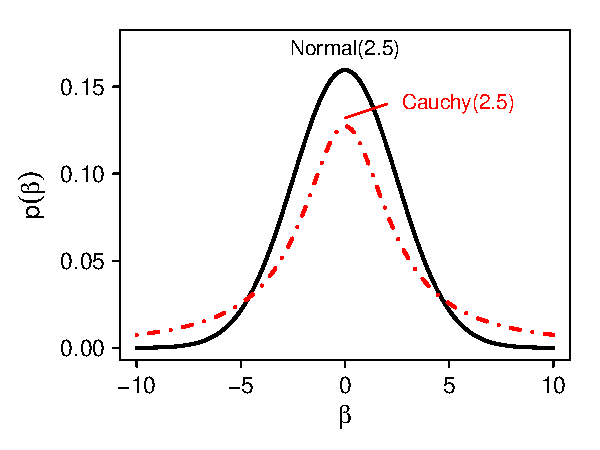
\includegraphics[scale = .8]{figs/illustrate-prior-density.pdf}
\caption{This figure compares the Normal(2.5) and Cauchy(2.5) prior distributions. Notice that the Cauchy distribution has a similar shape to a Normal distribution, but has much heavier tails. Substantively, this prior notes that the coefficient is likely close to zero (e.g. $|\beta| < 2$), but might be quite large (e.g., $|\beta| > 5$).}\label{fig:illustrate-prior-density}
\end{center}
\end{figure}

The posterior distribution is not easily available analytically, but one can easily use MCMC to simulate from the posterior distribution. \footnote{\citep{Gelmanetal2008} obtain standard errors of their estimates by simply calculating the curvature around the posterior mode. They note that although the entire posterior distribution can be computed using MCMC methods, ``it is desirable to have quick calculations that returns a point estimate of the regression coefficients and the standard errors'' (p. 1366). They note that this approximation ``works well in statistical practice and, in addition, recognizes the approximate nature of the model itself.'' However, our purpose is to accurately characterize the uncertainty of the estimates, and asymptotic approximations can underestimate credible intervals by quite a bit.} To facilitate this estimation, I have written an R function, \texttt{cauchy}, to obtain posterior simulations.\footnote{The R package \texttt{MCMCpack} offers some potential to sample from the posterior distribution via a Metropolis-Hastings algorithm with little custom software via the \texttt{MCMClogit()} function. However, the default proposal distribution relies on the large-sample covariance matrix for the parameter estimates. This covariance matrix, of course, is not useful since the variances for the separated variables are much too large. As far as I can tell, the contribution of the large-sample covariance matrix to the proposal distribution is not easily modified. For this reason, I have written custom samplers that use a Metropolis-Hastings algorithm to obtain posterior simulations.} Once a researcher has the MCMC simulations, she can obtain the $(1 - \alpha)100\%$ Bayesian credible interval for parameters by summarizing the simulations.

\section*{The Importance of the Prior}

Choosing a reasonable prior distribution is crucial for dealing with separation in a substantively meaningful manner. In many cases, the data (though the likelihood) swamp the contribution of the prior. However, in the case of separation such that $s_i$ perfectly predicts events, the likelihood determines the shape of the left-hand side of the posterior distribution and the prior (symmetric about zero) determines the shape of the right hand side of the posterior.

The likelihood has an ``S''-shape that approaches a limit of one as the parameter coefficient for the separating variable $s_i$ approaches infinity. Thus, for large values of the coefficient, the likelihood is essentially flat, which allows the prior distribution to drive the inferences. Thus the prior distribution is not an arbitrary choice made for computational convenience--but a choice that affects the inferences.

\subsection*{The Impact of the Prior in Theory}

Suppose that an explanatory variable $s_i$ perfectly predicts a binary outcome variable $y_i = 1$, such that whenever $s_i = 1$, $y_i = 1$, but when $s_i = 0$, $y_i$ might equal zero or one. \cite{AlbertAnderson1984} refer to this situation as quasicomplete separation. Suppose further an additional set of covariates $X_i$ and the analyst wishes to obtain plausible estimates of coefficients the model $Pr(y_i =1) = \text{logit}^{-1}(\alpha + \delta s_i + X_i \beta)$. It is easy to find plausible estimates of $\beta$ using the techniques discussed above (even maximum likelihood usually provides reasonable estimates of these parameters), but finding plausible estimates of $\alpha$ and $\delta$ proves more difficult because maximum likelihood suggests estimates of $-\infty$ and $+\infty$, respectively. In order to obtain a plausible estimate of $\delta$ (which will, in turn, provide a plausible estimate of $\alpha$), the researcher must introduce prior information into the model. My purpose here is to characterize how this prior information impacts the posterior distribution.

In the general situation, the analyst is interested in computing and characterizing the posterior distribution of the coefficient for $s_i$ given the data. Using Bayes' Rule, this posterior depends on the likelihood and the prior, so that $p(\delta, \beta | y) = p(y|\beta, \delta)p(\beta, \delta)$.\footnote{If we wanted only the posterior distribution of the scalar $\delta$, we could integrate out the parameter vector $\beta$, giving $p(\delta | y) = \int_{-\infty}^{\infty} p(y|\beta, \delta)p(\beta, \delta)d\beta$.} In particular, the analyst might have in mind a family of priors centered at and monotonically decreasing away from zero with varying scale $\sigma$, so that $p(\delta) = p(\delta | \sigma)$. Suppose that for a particular $\delta^* \geq 0$ the prior distribution is decreasing in $\delta$ at a decreasing rate. Intuitively, this assumption of a $\delta^*$ allows the result to generalize to many common distributions.\footnote{In particular, if the prior distribution is in the form of a double-exponential, which lacks ``shoulders,'' then $\delta^* = 0$. However, the most common prior distributions used in applied work, such as the normal, $t$, and Jeffreys', have ``shoulders'' such that $\delta^* > 0$. In this case, the exact curvature of the distribution in the region $[0, \delta^*]$ affects the relative impact of the prior.} 
Finally, suppose that the informativeness of the prior distribution depends on scale parameter $\sigma$ that is chosen by the researcher and ``flattens'' the prior $p(\delta) = p(\delta | \sigma)$, such that as $\sigma$ increases, the rate a which the prior descends to zero decreases.

\begin{restatable}{theorem}{impact}\label{thm:impact}
The impact of the researchers choice of $\sigma$ on the posterior distribution $p(\delta | y)$ is increasing in $\delta$ for $\delta> \delta^*$. 
\end{restatable}

In many cases, researchers summarize the posterior distribution by providing the 5th and 95th percentiles and a measure of centrality, such as the median.

\begin{quote}
\textsc{Practical Implication of Theorem \ref{thm:impact}:} Under quasicomplete separation where $x_i$ perfectly predicts $y_i = 1$, the prior has a small impact on the lower bound of the 90\% credible interval, a moderate impact on the measures of the location of the posterior (i.e., mean, median, and mode), and a large impact on the upper-bound of the credible interval.
\end{quote}

\subsection*{The Impact of the Prior in Practice}

To illustrate the impact of the prior on inferences when facing separation, I replicate a results from \cite{BarrilleauxRainey2014}, who are interesting in the effect of partisanship on governors' decisions to oppose the Medicaid expansion in their states under the Patient Protection and Affordable Care Act (ACA).\footnote{\cite{BarrilleauxRainey2014} use a logistic regression modeling the probability that a governor opposes the expansion using the following explanatory variables: the partisanship of the governor, the percent of the state's residents who are favorable toward the ACA, whether Republicans control the state legislature, the percent of the state that is uninsured, a measure of the fiscal health of the state, the Medicaid multiplier for the state, the percent of the state that is nonwhite, and the percent of the state that resides in a metropolitan area. See their paper for more details.} As the authors note, no Democrats opposed the expansion leading to a problem of separation. I use MCMC to simulate from the posterior using several different prior distributions, including Jeffreys' prior \citep{Zorn2005} and the Cauchy prior with scales of 1, 2.5, and 5 \citep{Gelmanetal2008}. While the choice of prior does not affect the conclusion about the \emph{direction} of the effect, it has a large impact on the conclusion about the \emph{magnitude} of the effect. This can be especially important when researchers are making claims about the substantive importance of their estimated effects (see \citealt{Rainey2014}, \citealt{Gross2014}, and \citealt{McCaskeyRainey2014}).

Figure \ref{fig:matters-post} shows the posterior distribution for the coefficient for the indicator of Republican governors. Notice that the different priors lead to different posterior distributions. Notice, in particular, that the choice of the prior has a large impact on the right-hand side of the posterior. More informative priors (e.g., Jeffrey's prior) lead to a more peaked posterior distribution that rules out very large effects. Less informative priors (e.g., Cauchy(2.5)) lead to the conclusion that even large effects are plausible. These differences affect the conclusions that the researchers draw about the likely magnitude of the effect.

\begin{figure}[H]
\begin{center}
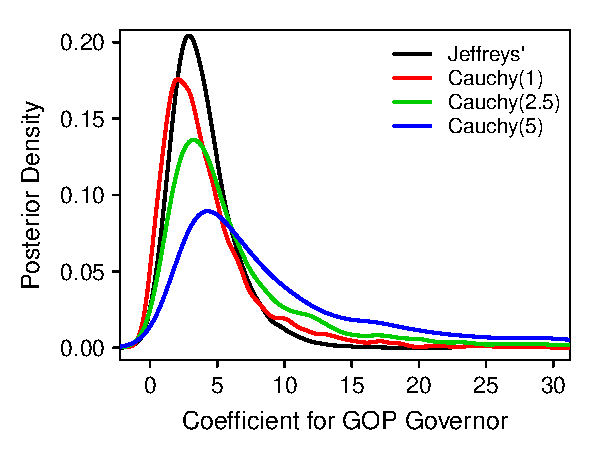
\includegraphics[scale = .8]{figs/matters-post.pdf}
\caption{This figure provides the posterior distribution for the coefficient of the indicator for GOP governors in the model offered by \cite{BarrilleauxRainey2014}. Notice that the location and the spread of the posterior depend on the prior chosen, especially the right-hand side of the distribution.}\label{fig:matters-post}
\end{center}
\end{figure}

Figure \ref{fig:matters-ci} shows how the choice of prior impacts the 90\% credible interval. Notice that different prior distributions lead to different conclusions about the plausible values of the effect. In particular, different priors lead to different conclusions about the upper-bound on the plausible effect sizes. For example, Jeffreys' prior, the default proposed by \cite{Zorn2005} and \cite{HeinzeSchemper2002}, suggests the effect lies in the range $\beta_{\text{GOP Gov.}} \in [0.9, 8.4]$, with a posterior mean of 3.9. On the other hand, the less informative Cauchy(2.5) prior, the default proposed by \cite{Gelmanetal2008}, suggests the effect lies in the range $\beta_{\text{GOP Gov.}} \in [1.0, 22.5]$, with a posterior mean of 7.3. A simple change from one proposed default to another more than doubles the upper bound on the 90\% credible interval and almost doubles the posterior mean. Further, the Cauchy(5) prior, a plausible prior if one believes the effect might be large, produces the upper-bound on the 90\% credible interval from is more than four times larger than the upper-bound produced by Jeffrey's prior. The posterior mean from the Cauchy(5) prior is larger falls above the upper-bound from the 90\% credible interval from Jeffrey's prior.

\begin{figure}[H]
\begin{center}
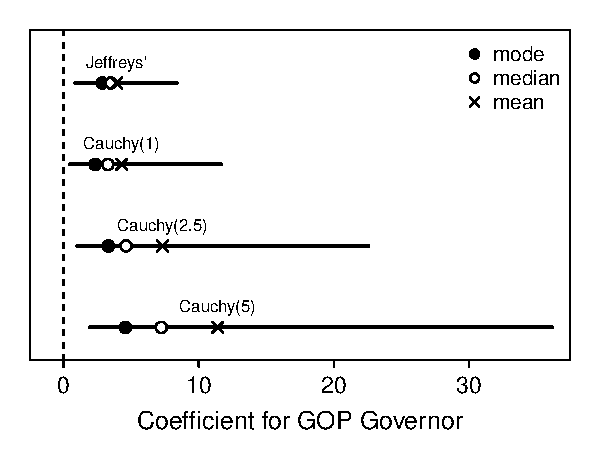
\includegraphics[scale = .8]{figs/matters-ci.pdf}
\caption{This figure provides the (equal-tailed) 90\% credible intervals for the coefficient of the indicator for GOP governors in the model offered by \cite{BarrilleauxRainey2014}. Notice that the location and the spread of the posterior depend on the prior chosen, especially the right-hand side of the distribution. Note that Jeffrey's prior, suggested by \cite{Zorn2005}, is the most informative of these priors, suggesting that a coefficient smaller than about 10 is quite unlikely. On the other hand, credible interval using the Cauchy(2.5) prior, as suggested by \cite{Gelmanetal2008}, is about \emph{twice} as wide as the credible interval from Jeffreys' prior. Finally, notice that the Cauchy(5) prior--a plausible prior if the researcher believes the effect might be large--produces a posterior mean larger than the upper bound of the 90\% credible interval using Jeffrey's prior.}\label{fig:matters-ci}
\end{center}
\end{figure}

This leads us to conclude that the choice of prior matters--it affects the inferences that we draw from the data. It is not sufficient to rely on the prior distribution designed as a default for other purposes. Instead, we must rely on prior distributions that represent actual prior information about the likely magnitude of the coefficients.


\section*{Choosing an Appropriate Prior Distribution}

Whilet is often sufficient to rely on default priors, this is not the case if one is interested in obtaining reasonable measures of uncertainty under separation. Indeed, I show above that the width of the 90\% credible interval and the posterior mean depend largely on the prior one chooses in the replication of \cite{BarrilleauxRainey2014}. This implies that researchers relying on default priors alone riskunder- or over-representing their confidence in the magnitude of the effect.

When facing separation, our goal is to choose a prior distribution that satisfies three properties:
\begin{enumerate}
\item Appropriately skeptical. As mentioned before, the prior distribution largely drives the right-hand side of the posterior distribution when $s_i$ perfectly predicts $y_i = 1$ and the left-hand side of the distribution when $s_i$ perfectly predicts $y_i = 0$. In this case, a non-central prior distribution in the direction of the separation has an especially large impact on the inferences. For this reason, I focus on prior distributions centered at zero to conservatively pool coefficients downward toward zero.
\item Allow plausible effects. The prior distribution should assign realistic prior probabilities to estimates that are \textit{a priori} plausible. 
\item Rule out implausible effects. The prior distribution should assigned essentially know prior probability to estimates that are \textit{a priori} implausible.
\end{enumerate}

\subsection*{Prior Predictive Distribution}

One method of assessing the reasonableness of the prior distribution is ``prior predictive checks,'' in which the researcher asks herself whether the prior distribution (combined with the model) produces a distribution for the data that matches her prior beliefs. Under the Bayesian framework, the researcher has a fully specified model $p(y_{new}|\theta)p(\theta)$ and can thus simulate data $y_{new}$ from the model prior to observing the data. The distribution of the unobserved outcome $y_{new}$ is given by $p(y_{new}) = \int p(y_{new} | \theta)p(\theta) d\theta$ \citep{Box1980}. In practice, this process involves Clarify-like simulation \citep{KingTomzWittenberg2000}, but rather than using the asymptotic posterior (e.g., $\beta_{sim} \sim N\left[\hat{\beta}^{mle}, I(\hat{\beta}^{mle})^{-1}\right]$), researchers simulate the model parameters from the prior distribution. Just as when using simulation to interpret the estimates, researchers can use simulation to interpret the prior distribution.

However, it is difficult to work with more than one dimension of the prior distribution at once and choosing the full prior distribution requires simultaneously choosing prior distributions for the $k + 1$ explanatory variables, as well as the relationships among these variables. But not all of this $k + 1$ dimensional distribution is of practical importance. Since the data swamp the prior for all but the separated coefficient, only the ``slice'' of the prior distribution with all other coefficients near their maximum likelihood estimates are relevant. I refer to this simplified focus as the \emph{partial} prior predictive distribution.

\subsection*{Partial Prior Predictive Distribution}

In many applications, the data swamp the prior so that changes in the prior distribution lead to only small changes in the inferences. In the case of separation, this is also the case, except for the separating variable in the direction of the separation. The likelihood makes a large contribution to the posterior for the non-separated coefficients and to the separated coefficient against the direction of the separation. However, the choice of the prior distribution has a large impact on the prior distribution for the separated coefficient in the direction of the separation.

Thus, in handling separation, we need to focusing on choosing reasonable prior distribution for the coefficient of the separating variable that assigned higher probabilities to more plausible estimates and lower probabilities to less plausible estimates.

For example, partisanship might have only a negligible effect on governors' decisions to oppose expansion. This is inconsistent with the hypothesis proposed by \cite{BarrilleauxRainey2014}, but it offers a \emph{plausible} alternative. On the other hand, we can \textit{a priori} rule out Democrats being 100\% likely to support the expansion and/or Republicans being 100\% likely to oppose--there is always some chance of Democratic governors opposing the expansion and Republican governors supporting it. However, the trick is to use substantive knowledge of the process to decide which effects are implausible large and which are not.

 the we need to focus on using the prior distribution to rule out only implausible values in the direction of the separation [ctk: I need to define the direction of the separation]. For example, if no Democratic governors oppose the expansion, then we do not need to worry about ruling out large \textit{positive} effects for Democratic partisanship, since the likelihood component of the model effectively rules out these implausible effects (e.g., large positive effects of Democratic partisanship on the probability of opposing the expansion are unlikely to generate data in which no Democrat opposes the expansion). We do, on the other hand, need to worry about ruling out the large \textit{negative} effects, since the likelihood cannot effectively rule out the implausibly large negative effects (e.g., the larger the negative effect, the more likely the observed separation will occur). See Theorem \ref{thm:impact} for a more formal treatment of this intuition.

Steps for choosing a reasonable prior for $\beta_s$.
\begin{enumerate}
\item Estimate the model coefficient using maximum likelihood, giving the coefficient vector $\hat{\beta}^{mle}$. Include the separating variable $s_i$ in the model. Of course, this leads to implausible estimates for $\beta_s$, but our goal here is to choose reasonable values at which to fix the other parameters. 
\item Choose a prior distribution $p(\beta_s)$ for the separating variable $s$. 
\item Choose a number of simulations $n_{sims}$ to perform (e.g., $n_{sims} \geq 1,000$) and for $i$ in 1 to $n_{sims}$ (e.g., $n_{sims} \geq 1,000$), do the following:
	\begin{enumerate}
	\item Simulate $\tilde{\beta}^{[i]}_s \sim p(\beta_s)$.
	\item Replace $\hat{\beta}_s^{mle}$ in $\hat{\beta}^{mle}$ with $\tilde{\beta}^{[i]}_s$, yielding the vector $\tilde{\beta}^{[i]}$.
	\item Calculate the store the quantity of interest $q^{[i]} = q\left(\tilde{\beta}^{[i]}\right)$. This quantity of interest might be a first-difference or risk-ratio, for example.
	\end{enumerate}
\item Summarize the simulations $q^{[i]}$ using quantiles, histograms, or density plots. If the prior is inadequate, then update the prior distribution $p(\beta_s)$.
\end{enumerate}

\section*{Application: Nuclear Proliferation and War}

I recent debate emerged in the conflict literature around the effect of nuclear weapons on the probability of war in a dyad. \cite{Rauchhaus2009} hypothesizes that ``[t]he probability of major war between two states will decrease if both states possess nuclear weapons (p. 262).'' Summarizing his empirical results, Rauchhaus writes:

\begin{quote} 
The hypotheses on nuclear symmetry find strong empirical support. The probability of a major war between two states is found to decrease when both states possess nuclear weapons (p. 269).
\end{quote}

Despite using the same data, \cite{BellMiller2014} claim that ``nonnuclear dyads are in fact no more likely to fight wars than nonnuclear dyads (p. 9).'' Their disagreement hinges, in part, on whether and how to handle separation, because no nuclear dyad in Rauchhaus data engage in war.\footnote{\cite{BellMiller2014} also disagree with a coding decision of \cite{Rauchhaus2009}, but that portion of their argument is less relevant to my purpose. Instead, my goal is to illustrate how one might choose a reasonable prior distribution and highlight the importance of the choice of prior.} \cite{Rauchhaus2009} ignores the separation and estimate that nonnuclear dyads are about 2.7 million times more likely to go to war than symmetric nuclear dyads. \cite{BellMiller2014}, on the other hand, use Jeffreys' (\citeyear{1946}) invariant prior, as suggested by \cite{Zorn2005}, and estimate that nonnuclear dyads are only about 1.6 times more likely to engage in war. Because these authors use very different prior distributions, they reach very different conclusions. This raises important questions. First, if we build a reasonable, informative prior distribution, does it support Rauchhaus' position of a meaningful effect or Bell and Miller's position of essentially no effect? Second, how robust is the conclusion to a range of more and less informative prior distributions?

\subsection*{Prior}

The first step in dealing with the separation in a principled manner is to choose a prior distribution. As discussed about, choose a prior distribution for a multivariate model is a complicated decision. However, the likelihood is highly informative about all coefficients except for the indicator of symmetric nuclear dyads (which perfectly predicts the absence of war and thus produces a estimate of minus infinity in theory and an implausibly large, negative estimates in practice). The likelihood is also highly informative about the estimate falling below zero, because these data would be extremely unlikely if nuclear weapons made war \emph{more} likely. However, the prior must crucially prior information about the plausibility of certain negative effects of nuclear weapons on the probability of conflict. 

To choose a reasonable prior, I follow steps 1-4 above to generate a partial prior predictive distribution for the risk-ratio discussed in detail by \cite{BellMiller2014}. I experimented with a range of prior distributions, from a varieties of families, but settled on the normal family. After some experimentation, I selected a normal distribution with mean zero and standard deviation 4.5 serve as an informative prior and represent my own prior beliefs. To evaluate the robustness of any statistical claims to the choice of prior. I also selected a normal distribution with mean zero and standard deviation 2 to serve as a skeptical prior that might be held by someone who beliefs that any pacifying effects of nuclear weapons is small or nil. Finally, I selected a normal distribution with mean zero and standard deviation 2 to serve as a optimistic prior that might be held by someone who beliefs that the pacifying effects of nuclear weapons might be quite large. Because the likelihood is highly informative about the other parameters in the model, I place an (improper) flat prior for these parameters. Figure \ref{fig:bm-pppd-hist} shows the PPPDs for the informative, skeptical, and enthusiastic prior distributions, along with Gelman's suggested default Cauchy prior centered at zero with scale 2.5. For convenience, Table \ref{tab:bm-pppd-deciles} provides the deciles of the PPPDs shown in Figure \ref{fig:bm-pppd-hist}. 

\begin{figure}[H]
\begin{center}
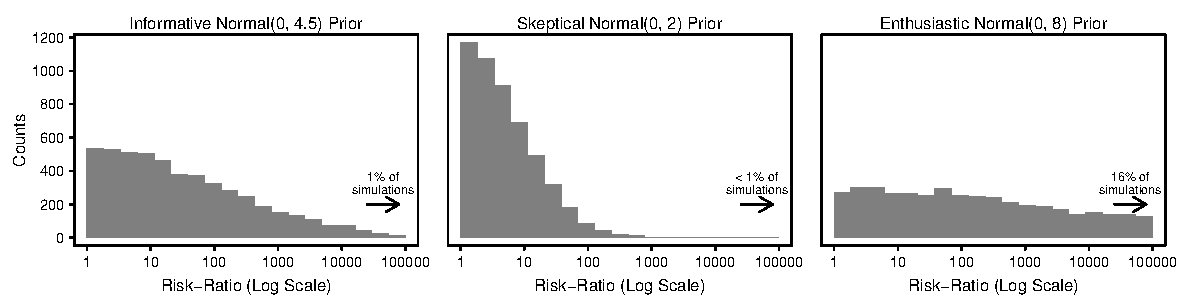
\includegraphics[scale = .8]{figs/bm-pppd-hist.pdf}
\caption{This figure shows the partial prior predictive distribution for the risk-ratio of war in nonnuclear to nuclear dyads. The risk-ratio is tells us how many times more likely war is in non-nuclear dyads compared to nuclear dyads. Notice that the informative prior treats effects smaller than 100 as plausible, but essentially rules out effects larger than 10,000. Gelman's suggested default places more weight closer to zero and more weight above 10,000. The skeptical prior essentially rules out effects larger than 100, while the enthusiastic prior treats effects between 1 and 100,000 as essentially equally likely.}\label{fig:bm-pppd-hist}
\end{center}
\end{figure}

% latex table generated in R 3.1.1 by xtable 1.7-3 package
% Sun Oct  5 07:07:18 2014
\begin{table}[H]
\centering
{\scriptsize
\begin{tabular}{|cccccccccc|}
  \hline
 & 10\% & 20\% & 30\% & 40\% & 50\% & 60\% & 70\% & 80\% & 90\% \\ 
  \hline
Informative Normal(0, 4.5) Prior &       1.7 &       3.1 &       5.6 &      10.3 &      19.5 &      44.1 &      98.8 &     296.9 &   1,577.7 \\ 
  Skeptical Normal(0, 2) Prior &       1.3 &       1.7 &       2.2 &       2.9 &       3.9 &       5.4 &       8.3 &      13.2 &      26.7 \\ 
  Enthusiastic Normal(0, 8) Prior &       2.9 &       8.1 &      24.7 &      76.5 &       256 &     987.6 &   5,300.9 &  42,466.7 & 643,954.6 \\ 
   \hline
\end{tabular}
}
\caption{This table provides the deciles prior predictive distribution for the 
                  risk-ratio of war in nonnuclear and nuclear dyads. The risk-ratio is 
                  tells us how many times more likely war is in non-nuclear dyads compared 
                  to nuclear dyads. Notice that that the, informative prior suggests a median 
                  risk-ratio of about 20, which is a large, but plausible effect. The skeptical prior suggests a median 
                  ratio of about 4 and the enthusiastic prior suggests a median ratio of over 
                  200.} 
\label{tab:bm-pppd-deciles}
\end{table}


Notice that the skeptical prior suggests that risk-ratios above and below 4 are equally likely (i.e., 50th percentile of the PPPD is 3.9), while the enthusiastic prior suggests that effects above and below 220 are equally likely. The informative prior, on the other hand, suggests (more reasonably, in my view) that the effect is equally likely to fall above and below 20. These three prior distributions (along with the defaults suggested by \cite{Zorn2005} and \cite{Gelmanetal2008}) provide a range of distributions to represent a range of prior beliefs.

\subsection*{Posterior}

Figure \ref{fig:bm-posterior-density} shows the posterior distributions from the informative, skeptical, enthusiastic, and two default prior distributions. The areas shaded grey indicate the 90\% highest posterior density (HPD) intervals, akin to a 90\% confidence interval.\footnote{Obviously, we could define many intervals that have 90\% chance of containing the true parameter. However, the HPD interval is theoretically appealing because it is the \emph{shortest} of these intervals. See \citet[esp. pp. 48-51]{Gill2008} and \citet[esp. p. 448]{CasellaBerger2003}.} Notice that the location (e.g., peak or model), shape, scale, and HPD interval depend on the choice of prior. While the magnitude of these effects cannot be easily interpreted, notice that the Gelman's suggested default prior is somewhat similar to the informative prior, but Zorn's suggested default is quite similar to the \emph{skeptical} prior. Thus, when dealing with separation, these distributions illustrate that the prior is not an unimportant choose. Instead, it is critical to obtaining reasonable inferences.

\begin{figure}[H]
\begin{center}
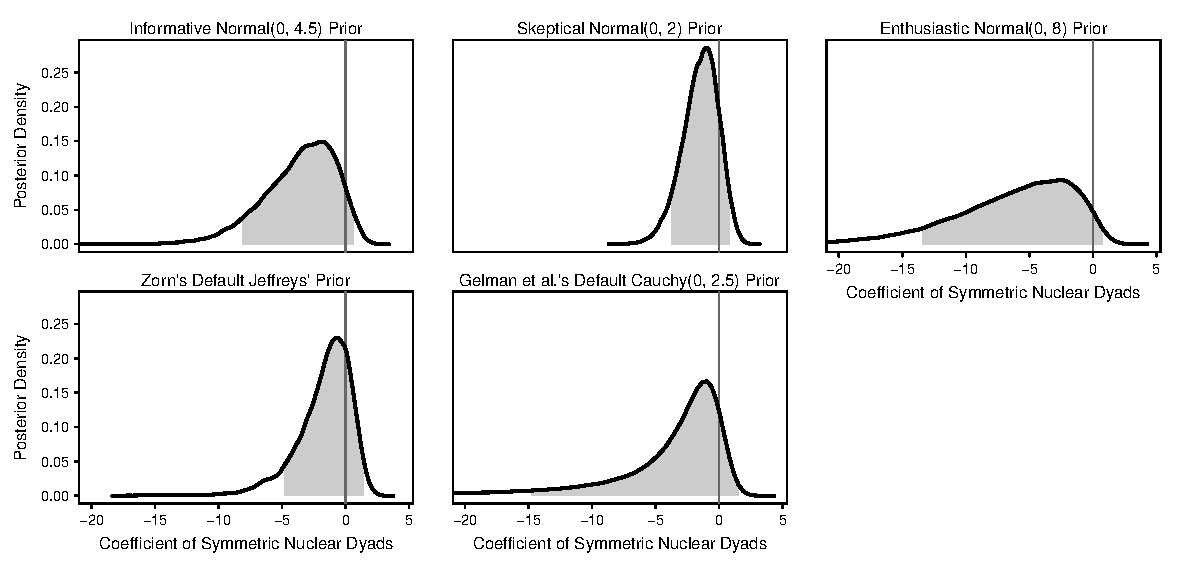
\includegraphics[scale = .8]{figs/bm-posterior-density.pdf}
\caption{This figure shows the posterior distribution for the logit coefficient using each of the five prior distributions.  The grey shading indicates the 90\% highest posterior density (HPD) . Notice that the choice of prior has a large effect on the inferences. For example, the enthusiastic prior suggests the ratio might be as large as -13, while the skeptical prior suggests the ratio might be as large as -4. Importantly, notice the similarity between the posterior from Zorn's suggested default and the skeptical prior, in terms of their peak (i.e., mode), shape, and highest posterior density.}\label{fig:bm-posterior-density}
\end{center}
\end{figure}

I now turn to the posterior distribution of the risk-ratios--the key quantity of interest in the debate between \cite{BellMiller2014} and \cite{Rauchhaus2009}. Figure \ref{fig:bm-rr} presents the posterior medians and the 90\% HPD intervals for each prior. While an initial glance at the figure shows substantial variation in the point estimates and the width of the intervals, notice that these are plotted on the log scale (otherwise the wider intervals dominate the plot). Notice that the informative prior suggests the true risk-ratio has about a 90\% chance of falling between about 0.1 and about 2000, with a posterior median of about 25.\footnote{It is worth pointing out that these wide confidence interval suggest that, although the HPD intervals overlap zero, these data do not warrant a conclusion of ``no effect'' (see \citealt{Rainey2014}).} The skeptical prior, on the other hand, suggests the risk-ratio has about a 90\% chance of falling between 0.1 and 30, with a posterior median of about 4. The enthusiastic prior suggests the risk-ratio has about a 90\% chance of falling between 0.1 and 500,000. The inferences from these priors are \emph{very} different. Further, while the 90\% HPD interval is \emph{much} narrower than the informative prior, and the posterior median of Zorn's suggested default prior is smaller than the \emph{skeptical} prior. For out particular application, Gelman's suggested default more closely matches the informative prior, but in another application, Zorn's suggested default might correspond more closely to a carefully-chosen, informative prior.

%\begin{figure}[H]
%\begin{center}
%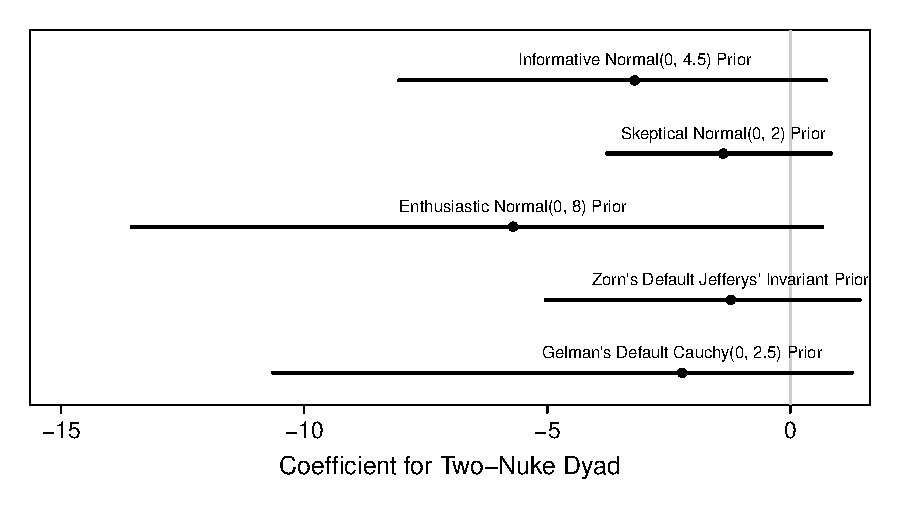
\includegraphics[scale = .8]{figs/bm-coef.pdf}
%\caption{}\label{fig:bm-coef}
%\end{center}
%\end{figure}

\begin{figure}[H]
\begin{center}
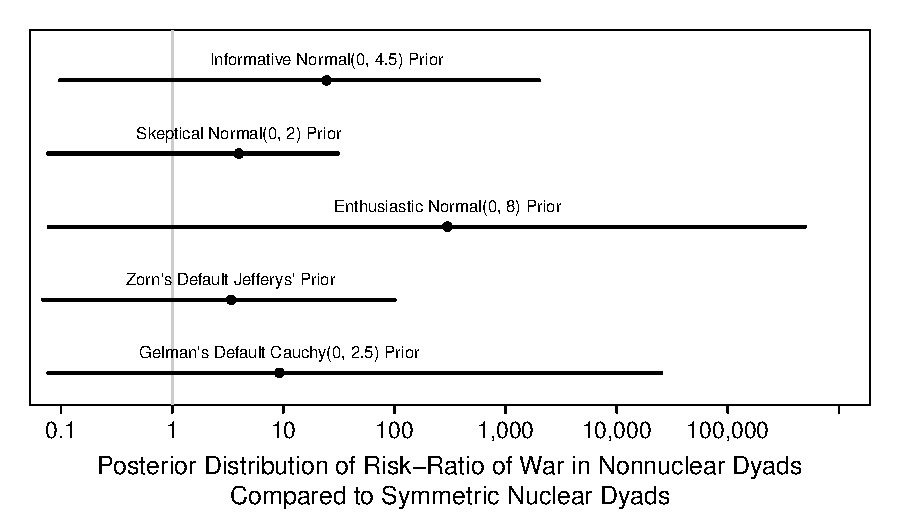
\includegraphics[scale = .8]{figs/bm-rr.pdf}
\caption{This figure shows the posterior median and 90\% highest posterior density (HPD) for the risk-ratio using each of the five prior distributions \emph{on the log scale}. Notice that the choice of prior has a huge effect on the inferences about the risk-ratio. For example, the skeptical prior suggests the ratio might be as large as 31, while the enthusiastic prior suggests the ratio might be as large as 500,000. Also, notice that the posterior median from Zorn's proposed default prior is \emph{smaller} than the posterior median from the skeptical prior.}\label{fig:bm-rr}
\end{center}
\end{figure}

%% latex table generated in R 3.1.1 by xtable 1.7-3 package
% Mon Oct  6 05:01:40 2014
\begin{table}[H]
\centering
{\scriptsize
\begin{tabular}{|cccc|}
  \hline
 & Lower-Bound of 90\% HPD & Posterior Median & Upper-Bound of 90\% HPD \\ 
  \hline
Informative Normal(0, 4.5) Prior &       0.1 &      24.5 &   1,986.4 \\ 
  Skeptical Normal(0, 2) Prior &       0.1 &         4 &      31.2 \\ 
  Enthusiastic Normal(0, 8) Prior &       0.1 &     299.2 & 499,043.2 \\ 
  Zorn's Default Jeffreys' Prior &       0.1 &       3.4 &     100.2 \\ 
  Gelman et al.'s Default Cauchy(0, 2.5) Prior &       0.1 &       9.2 &  25,277.4 \\ 
   \hline
\end{tabular}
}
\caption{This table provides lower- and upper-bounds for the 90% HPD and posterior medians 
              for the five prior distributions I consider.} 
\label{tab:bm-pppd-deciles}
\end{table}


Finally, I use the posterior distributions from each prior to calculate the probability that the presence of nuclear weapons make war less likely (i.e., the probability that the risk-ratios show in Figure \ref{fig:bm-rr} are greater than one). Recall Rauchhaus' hypothesis that nuclear weapons decrease the chance of war. These probabilities can be thought of as the probability that Rauchhaus' hypothesis is correct. Following the standard of $p-value \leq 0.05$ as offering strong evidence against the null, it is reasonable to take $Pr(RR > 1) \geq 0.95$ as strong evidence for the research hypothesis. Figure \ref{fig:bm-rr} shows the probability that the hypothesis is correct for each prior distribution. Notice that while only the enthusiastic prior falls above the 0.95 standard, the evidence for the claim is at least suggestive. Perhaps most importantly for my purposes, Zorn's suggested default leads to the \emph{least} evidence in favor of Rauchhaus' hypothesis--even the skeptical prior provides more evidence for Rauchhaus' claim.

\begin{figure}[H]
\begin{center}
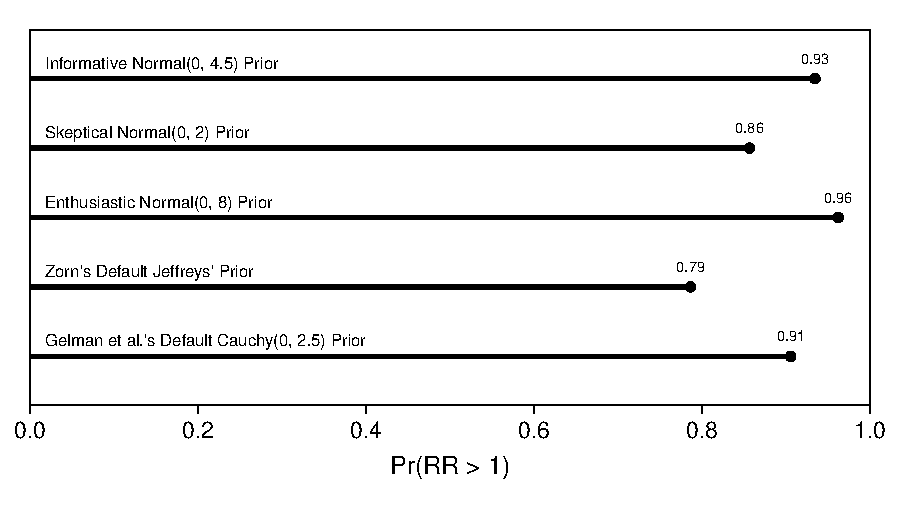
\includegraphics[scale = .8]{figs/bm-pr-hypothesis.pdf}
\caption{This figure shows the posterior probability of the hypothesis that nonnuclear dyads are \emph{more} likely to engage in war than symmetric nuclear dyads for each of the five prior distribution. From a hypothesis testing perspective, the evidence for the hypothesis is borderline or suggestive for each prior. However, notice that the skeptical prior, perhaps held by a skeptical researcher who believes the pacifying effect of nuclear weapons is small or nil, yields \emph{greater} evidence for the hypothesis than Jeffreys' invariant prior suggested as a default by \cite{Zorn2005}.}\label{fig:bm-pr-hypothesis}
\end{center}
\end{figure}

\subsection*{Implications}

This reanalysis shows how much the choice of prior can matter for substantive conclusions. Even the predominant default priors used to deal with separation can provide very different inferences than a carefully-chosen, informative prior. For this example, Zorn's default prior suggested a point estimate about seven times smaller and a 90\% HPD interval about 20 times narrower than the informative prior.

What does this mean for applied researchers? I suggest two implications.
\begin{enumerate}
\item When facing separation, the choice of prior matters. Researchers must carefully choose a prior that represents actual prior information, otherwise, the point and interval estimates will be too large.
\item In addition to carefully choosing an informative prior, researchers should show how the inferences change for a range of prior distributions. In the debate between \cite{BellMiller2014} and \cite{Rauchhaus2009}, the choice of prior almost completely drives the inferences about the likely magnitude of the risk-ratio. Thus, to the extent that there is disagreement about the prior, there will be disagreement about the results.
\end{enumerate}

\clearpage
\bibliographystyle{apsr_fs}
\bibliography{/Users/carlislerainey/Dropbox/papers/bibliography/bibliography.bib}

\clearpage
\begin{appendix}
\begin{center}
\LARGE{\textbf{Online Appendix}}\vspace{4mm}
\end{center}

\section*{Proof of Theorem \ref{thm:impact}}

\begin{assumption}[Separation]
Suppose quasicomplete separation such that $s_i$ perfectly predicts $y_i = 1$. 
\end{assumption}

\begin{assumption}[Prior Shape]
Suppose that the researcher computes the posterior distribution $p(\beta | y) = p(y | \beta)p(\beta)$ such that for a particular $\beta^* \geq 0$ the prior distribution is decreasing at a decreasing rate.
\end{assumption}

Intuitively, this assumption of a $\beta^*$ allows the result to generalize to a range of common distributions. In particular, if the prior distribution is in the form of a double-exponential, which lacks ``shoulders,'' then $\beta^* = 0$. However, the most common prior distributions used in applied work, such as the normal, $t$, and Jeffreys', have ``shoulders'' such that $\beta^* > 0$. In this case, the exact curvature of the distribution in the region $[0, \beta^*]$ affects the relative impact of the prior.

\begin{assumption}[Scale Parameter]
Suppose finally the that informativeness of the prior distribution depends on scale parameter $\sigma$ ``flattens'' the prior $p(\beta) = p(\beta | \sigma)$, such that as $\sigma$ increases, the rate a which the prior descends to zero decreases.
\end{assumption}

$\sigma$ is chosen by the researcher based on prior information about the likely values of the coefficients.

Before proving Theorem \ref{thm:impact}, it is helpful to show several initial results.

\begin{lemma}\label{thm:L1}
$\dfrac{\partial p(y | \beta)}{\partial \beta} > 0$ for all $\beta$. 
\end{lemma}

\begin{proof}[Proof of Lemma \ref{thm:L1}]
The quantity $p(y | \beta)$ is the probability of observing $y$ (i.e., an outcome variable separated by $s$). Increasing values of $\beta$ make this separation increasingly likely. Thus, $p(y | \beta)$ is increasing in $\beta$ so that $\dfrac{\partial p(y | \beta)}{\partial \beta} > 0$. 
\end{proof}

\begin{lemma}\label{thm:L2}
$p(\beta | \sigma) > 0$ for all $\beta$.
\end{lemma}

\begin{proof}[Proof of Lemma \ref{thm:L2}]
The quantity $p(\beta | \sigma)$ is a probability distribution defined to have support over the real line and thus $p(\beta | \sigma) > 0$ for all $\beta$. 
\end{proof}

\begin{lemma}\label{thm:L3}
$p(y | \beta) > 0$ for all $\beta$.
\end{lemma}

\begin{proof}[Proof of Lemma \ref{thm:L3}]
The quantity $p(y | \beta)$ is a probability and thus bounded between zero and one. As long as data lie within the support of the probability model, this quantity lies strictly above zero. Since the theorem defines the data as such, $p(y | \beta) > 0$.
\end{proof}

\begin{lemma}\label{thm:L4}
$\dfrac{\partial^2 p(\beta | \sigma)}{\partial \beta \partial \sigma}$ for $\beta > \beta^*$.
\end{lemma}

\begin{proof}[Proof of Lemma \ref{thm:L4}]
By assumption, the prior density is decreasing at a decreasing rate in $\beta$ for all $\beta > \beta^*$. Also by assumption, the scale parameter $\sigma$ controls the rate at which $\beta$ decreases such that increasing $\sigma$ leads to a slower rate of decrease. These two assumptions together imply that $\dfrac{\partial^2 p(\beta | \sigma)}{\partial \beta \partial \sigma}$ for $\beta > \beta^*$.
\end{proof}

Now recall Theorem \ref{thm:impact}:

\impact*

\begin{proof}[Proof of Theorem \ref{thm:impact}]
To show that the effect of $\sigma$ is increasing in $\beta$, I simply need to show that $\dfrac{\partial^2 p(\beta | y)}{\partial \beta \partial \sigma} > 0$ for $\beta > \beta^*$. 

Recall that the posterior $p(\beta | y)$ is proportional to the likelihood $p(y | \beta)$ times the prior $\beta(\beta | \sigma)$, so that $p(\beta | y) \propto p(y|\beta)p(\beta | \sigma)$. First, we can use the product rule to obtain the derivative of $p(\beta | y)$ so that 

\begin{equation}\nonumber
\dfrac{\partial p(\beta | y)}{\partial \beta} \propto \dfrac{\partial p(y | \beta)}{\partial \beta} p(\beta | \sigma) + p(y | \beta)\dfrac{\partial p(\beta | \sigma)}{\partial \beta \partial}\text{}.
\end{equation}

\noindent Only the final term involves $\sigma$, so we can easily obtain the desired derivative

\begin{equation}\label{eqn:cross-partial}
\dfrac{\partial^2 p(\beta | y)}{\partial \beta \partial \sigma} \propto \overbrace{\dfrac{\partial p(y | \beta)}{\partial \beta}}^{\text{Lemma 1}:~+} \overbrace{p(\beta | \sigma)}^{\text{Lemma 2}:~+} + \overbrace{p(y | \beta)}^{\text{Lemma 3}:~+} \overbrace{\dfrac{\partial^2 p(\beta | \sigma)}{\partial \beta \partial \sigma}}^{\text{Lemma 4}:~+}\text{.}
\end{equation}

\noindent Each term on the right-hand side of Equation \ref{eqn:cross-partial} is positive  for $\beta > \beta^*$ (Lemmas 1-4), so that $\dfrac{\partial^2 p(\beta | y)}{\partial \beta \partial \sigma} > 0$ for $\beta > \beta^*$.

\end{proof}

\end{appendix}
\end{document}



